%
\hsection{\crowsFoot{K}{M1}{L}{OM}}%
\label{sec:rm:kl}%
%
\begin{figure}%
\centering%
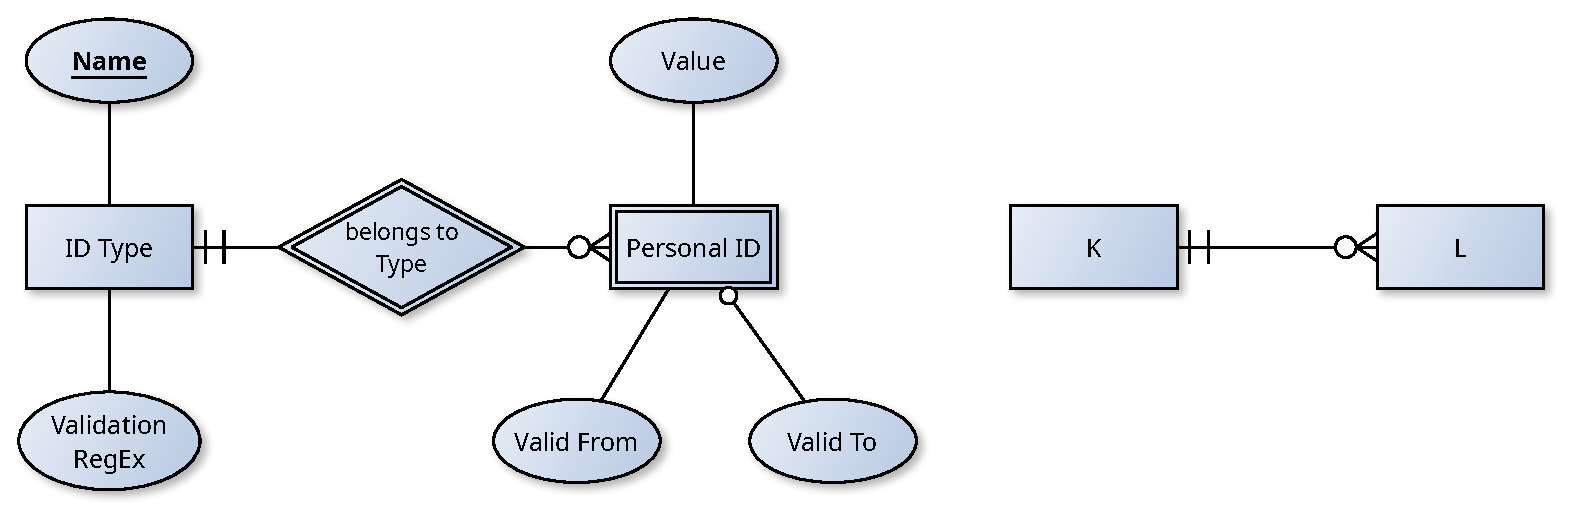
\includegraphics[width=0.97\linewidth]{\currentDir/KL}%
\caption{We encountered the \crowsFoot{K}{M1}{L}{OM} relationship pattern in \cref{fig:erdPerson4}.}%
\label{fig:rm:kl}%
\end{figure}%
%
\gitSQLAndOutput{\databasesCodeRepo}{conceptualToRelational}{KL_tables.sql}{relationships}{}{}{postgres.sh}{KL_tables}{%
The realization of a \crowsFoot{K}{M1}{L}{OM} conceptual relationship.%
}%
\gitSQLAndOutput{\databasesCodeRepo}{conceptualToRelational}{KL_insert_and_select.sql}{relationships}{}{}{postgres.sh}{KL_insert_and_select}{%
Inserting into and selecting data from the realization of an \crowsFoot{K}{M1}{L}{OM} conceptual relationship given in \cref{lst:KL_tables}.%
}%
%
\gitExecPath{\databasesCodeRepo}{conceptualToRelational}{../_scripts_/db_table_to_latex_table.sh relationships k kid;x}{cdtrmTableK}%
\gitExecPath{\databasesCodeRepo}{conceptualToRelational}{../_scripts_/db_table_to_latex_table.sh relationships l lid;fkkid;y}{cdtrmTableL}%
%
\begin{figure}%
\centering%
\floatSep%
\input{\cdtrmTableK}%
\floatSep%
\input{\cdtrmTableL}%
\floatSep%
\caption{The contents of the the two tables in the implementation of the \crowsFoot{K}{M1}{L}{OM} conceptual relationship after executing \cref{lst:KL_insert_and_select}.}%
\label{fig:rm:kl:tables}%
\end{figure}%
%
We have the two entity types~K and~L.
Each entity of type~K may be connected to zero, one, or multiple entities of type~L.
Each entity of type~L is connected to exactly one entity of type~K.

We already encountered this relationship pattern in back in \cref{fig:erdPerson4}, when we modeled the relationship between the entity types~\emph{Personal~ID} and~\emph{ID~Type}.
We found that there can be many different types of IDs, including the Chinese~IDs~(中国公民身份号码), passports, visas, or even mobile phone numbers.
For each such type, we may have zero, one, or many personal~ID records stored in our \db.
Each personal~ID, however, must always belong to exactly one ID~type.
This is illustrated in \cref{fig:rm:kl}.

We need a table~\sqlil{k} for the entities of type~K and a table~\sqlil{l} for the entities of type~L.
We call the primary key for table~\sqlil{k} \sqlil{kid} and also add the example attribute~\sqlil{x}.
The primary key for table~\sqlil{l} be~\sqlil{lid} and we again provide the example attribute~\sqlil{y}.
Every row of table~\sqlil{l} must be related to exactly one row of table~\sqlil{k}.
The three table solution from the \crowsFoot{E}{O1}{F}{OM} scenario therefore makes no sense:
The third table could never have few rows, it would always have exactly as many rows as~\sqlil{l}.

The sensible solution is to add a foreign key column to table~\sqlil{l} that references the primary key of table~\sqlil{k}, as shown in \cref{lst:KL_tables}.
Since the relationship is mandatory, the column must be~\sqlil{NOT NULL}.
It does not need to be unique, because each row in table~\sqlil{k} can be related to arbitrarily many rows in~\sqlil{l}.

We insert some data into this structure in \cref{lst:KL_insert_and_select}.
We can first create the rows for table~\sqlil{k}, because their relationship to rows in table~\sqlil{l} is optional.
Then we insert rows in table~\sqlil{l}.
For each of them, we must provide a valid value for the column~\sqlil{fkkid}, i.e., for the foreign key to table~\sqlil{k}.
The value in this column must match one existing value in column~\sqlil{kid} of table~\sqlil{k}.
The reason is that each row in table~\sqlil{l} must be related to exactly one row in table~\sqlil{k}.
Thus, providing~\sqlil{NULL} as~\sqlil{fkkid} is not possible.
The contents of the tables~\sqlil{k} and~\sqlil{l} after inserting the data are shown in \cref{fig:rm:kl:tables}.

It is impossible to add a row to table~\sqlil{l} without providing an existing value of the primary key attribute~\sqlil{id} of table~\sqlil{k} for the foreign key column~\sqlil{k}.
In other words, because of the \sqlil{REFERENCES} and the \sqlil{NOT NULL} constraint, each row in table~\sqlil{l} must reference exactly one row in table~\sqlil{k}.
It cannot reference more than one row, because the atttribute~\sqlil{k} can only take on a single value.
In turn, the rows in table~\sqlil{k} can be referenced by arbitrarily many rows in table~\sqlil{l}:
maybe by no row at all, maybe by one, maybe be hundreds.
This is exactly the meaning of the \inQuotes{optionally-many} relationship end pointing towards entity type~L.
In \cref{lst:KL_insert_and_select}, we insert some rows into both tables and combine the data together using a single \sqlilIdx{INNER JOIN}.%
%
\FloatBarrier%
\endhsection%
%
